\documentclass[tikz,border=12pt]{standalone}
\usepackage[T1]{fontenc}
\usepackage{lmodern}
\usepackage{amsmath}
\usepackage{graphicx}
\usetikzlibrary{arrows.meta,positioning,fit,calc,backgrounds}

\begin{document}
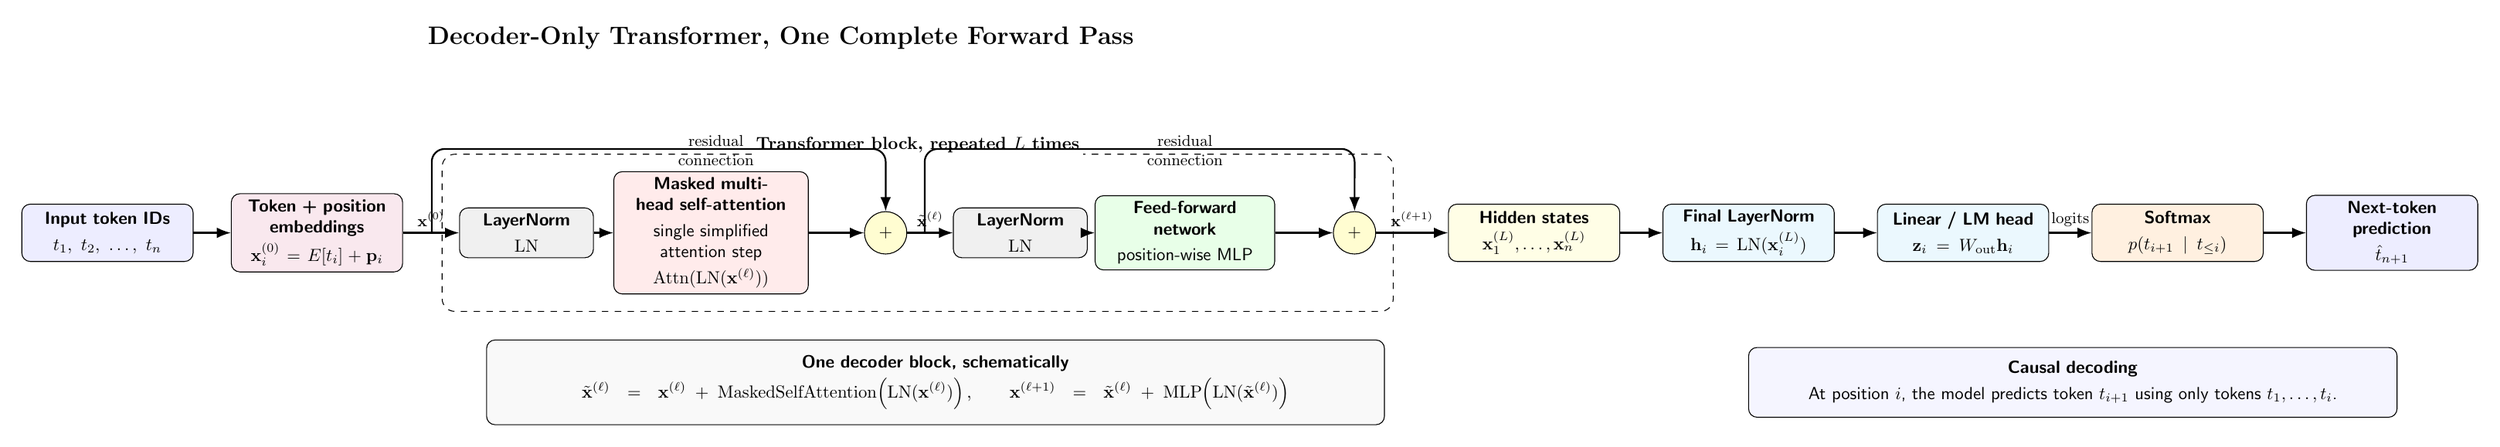
\begin{tikzpicture}[
    scale=0.82,
    every node/.style={transform shape},
    font=\sffamily,
    >=Latex,
    arrow/.style={->, thick},
    skiparrow/.style={->, thick, rounded corners=6pt},
    box/.style={
        draw,
        rounded corners=4pt,
        align=center,
        minimum height=1.15cm,
        minimum width=3.4cm,
        text width=3.2cm
    },
    smallbox/.style={
        draw,
        rounded corners=4pt,
        align=center,
        minimum height=1.0cm,
        minimum width=2.6cm,
        text width=2.45cm
    },
    inputbox/.style={
        box,
        fill=blue!7
    },
    embedbox/.style={
        box,
        fill=purple!9
    },
    normbox/.style={
        smallbox,
        fill=gray!12
    },
    attnbox/.style={
        box,
        fill=red!8,
        minimum width=3.9cm,
        text width=3.65cm
    },
    addbox/.style={
        circle,
        draw,
        fill=yellow!18,
        minimum size=0.85cm,
        inner sep=0pt,
        font=\bfseries
    },
    mlpbox/.style={
        box,
        fill=green!9,
        minimum width=3.6cm,
        text width=3.35cm
    },
    outbox/.style={
        box,
        fill=cyan!8
    },
    probbox/.style={
        box,
        fill=orange!12
    },
    dashedbox/.style={
        draw,
        dashed,
        rounded corners=6pt,
        inner sep=8pt
    }
]

% Title
\node[font=\bfseries\Large] (title) at (13.5,3.9) {Decoder-Only Transformer, One Complete Forward Pass};

% Input sequence
\node[inputbox] (tokens) at (0,0) {\textbf{Input token IDs}\\[1mm]
$t_1,\ t_2,\ \ldots,\ t_n$};

% Embedding
\node[embedbox] (embed) at (4.2,0) {\textbf{Token + position embeddings}\\[1mm]
$\mathbf{x}_i^{(0)}
=
E[t_i]+\mathbf{p}_i$};

% Transformer block internals
\node[normbox] (ln1) at (8.4,0) {\textbf{LayerNorm}\\[1mm]
$\mathrm{LN}$};

\node[attnbox] (attn) at (12.1,0) {\textbf{Masked multi-head self-attention}\\[1mm]
single simplified attention step\\[1mm]
$\mathrm{Attn}(\mathrm{LN}(\mathbf{x}^{(\ell)}))$};

\node[addbox] (add1) at (15.6,0) {$+$};

\node[normbox] (ln2) at (18.3,0) {\textbf{LayerNorm}\\[1mm]
$\mathrm{LN}$};

\node[mlpbox] (mlp) at (21.6,0) {\textbf{Feed-forward network}\\[1mm]
position-wise MLP};

\node[addbox] (add2) at (25.0,0) {$+$};

% Output of repeated block
\node[box, fill=yellow!10, minimum width=3.4cm, text width=3.2cm] (blockout) at (28.6,0) {\textbf{Hidden states}\\[1mm]
$\mathbf{x}^{(L)}_1,\ldots,\mathbf{x}^{(L)}_n$};

% Final norm and LM head
\node[outbox] (finalln) at (32.9,0) {\textbf{Final LayerNorm}\\[1mm]
$\mathbf{h}_i=\mathrm{LN}(\mathbf{x}_i^{(L)})$};

\node[outbox] (lmhead) at (37.2,0) {\textbf{Linear / LM head}\\[1mm]
$\mathbf{z}_i=W_{\mathrm{out}}\mathbf{h}_i$};

\node[probbox] (softmax) at (41.5,0) {\textbf{Softmax}\\[1mm]
$p(t_{i+1}\mid t_{\le i})$};

\node[inputbox] (nexttoken) at (45.8,0) {\textbf{Next-token prediction}\\[1mm]
$\hat{t}_{n+1}$};

% Main arrows
\draw[arrow] (tokens.east) -- (embed.west);
\draw[arrow] (embed.east) -- node[above, font=\small] {$\mathbf{x}^{(0)}$} (ln1.west);
\draw[arrow] (ln1.east) -- (attn.west);
\draw[arrow] (attn.east) -- (add1.west);
\draw[arrow] (add1.east) -- node[above, font=\small] {$\tilde{\mathbf{x}}^{(\ell)}$} (ln2.west);
\draw[arrow] (ln2.east) -- (mlp.west);
\draw[arrow] (mlp.east) -- (add2.west);
\draw[arrow] (add2.east) -- node[above, font=\small] {$\mathbf{x}^{(\ell+1)}$} (blockout.west);
\draw[arrow] (blockout.east) -- (finalln.west);
\draw[arrow] (finalln.east) -- (lmhead.west);
\draw[arrow] (lmhead.east) -- node[above, font=\small] {logits} (softmax.west);
\draw[arrow] (softmax.east) -- (nexttoken.west);

% Residual connections
\coordinate (resstart) at ($(ln1.west)+(-0.55,0)$);
\coordinate (resmidone) at ($(add1.north)+(0,1.25)$);
\draw[skiparrow]
    (resstart)
    |- (resmidone)
    -- (add1.north);

\coordinate (resstarttwo) at ($(add1.east)+(0.35,0)$);
\coordinate (resmidtwo) at ($(add2.north)+(0,1.25)$);
\draw[skiparrow]
    (resstarttwo)
    |- (resmidtwo)
    -- (add2.north);

% Residual labels
\node[font=\small, align=center] at (12.2,1.65) {residual\\connection};
\node[font=\small, align=center] at (21.6,1.65) {residual\\connection};

% Repeated transformer block background
\begin{pgfonlayer}{background}
\node[dashedbox, fit=(ln1)(attn)(add1)(ln2)(mlp)(add2)] (blockfit) {};
\node[font=\bfseries, fill=white, inner sep=2pt] at ($(blockfit.north)+(0,0.18)$)
    {Transformer block, repeated $L$ times};
\end{pgfonlayer}

% Formula annotation under transformer block
\node[
    draw,
    rounded corners=4pt,
    align=center,
    fill=gray!5,
    minimum width=18.0cm,
    text width=17.7cm,
    minimum height=1.7cm
] (formula) at (16.6,-3.0) {
\textbf{One decoder block, schematically}\\[1mm]
$\displaystyle
\tilde{\mathbf{x}}^{(\ell)}
=
\mathbf{x}^{(\ell)}
+
\mathrm{MaskedSelfAttention}\!\left(\mathrm{LN}(\mathbf{x}^{(\ell)})\right),
\qquad
\mathbf{x}^{(\ell+1)}
=
\tilde{\mathbf{x}}^{(\ell)}
+
\mathrm{MLP}\!\left(\mathrm{LN}(\tilde{\mathbf{x}}^{(\ell)})\right)
$
};

% Small note under output
\node[
    draw,
    rounded corners=4pt,
    align=center,
    fill=blue!4,
    minimum width=13.0cm,
    text width=12.7cm,
    minimum height=1.4cm
] (note) at (39.4,-3.0) {
\textbf{Causal decoding}\\[1mm]
At position $i$, the model predicts token $t_{i+1}$ using only tokens $t_1,\ldots,t_i$.
};

\end{tikzpicture}
\end{document}